\chapter{PDF Renderer}
\thispagestyle{fancy}

Kapitel erstellt von Tim Hebbeler
\\
Der PDF-Renderer wurde als separate C++-Klasse entwickelt und ist in die Android App und den Server eingebunden.

Im Laufe der Entwicklung wurden die Bibliotheken \href{https://poppler.freedesktop.org/}{Poppler} und \href{http://mupdf.com/}{MuPDF} untersucht. Das Projekt Poppler ist eine unter der GPL stehende Bibliothek und basiert auf \href{https://de.wikipedia.org/wiki/Xpdf}{Xpdf}. Poppler bietet schon ein Qt-Binding, doch leider liegt der Fokus auf unixartige Betriebssysteme und nicht auf der Plattformunabhängigkeit \footnote{\url{https://de.wikipedia.org/wiki/Poppler}}. Die PDF Darstellung wird aber auf verschiedenen Plattform, wie Android, dem Raspberry Pi und Windows benötigt, deshalb konnte Poppler nicht verwendet werden.
Die Wahl fiel deshalb auf MuPdf von der Firma Artifex Software, Inc. ,welches unter der AGPLv3 steht. Diese Bibliothek bieten kein Qt-Bindung, doch existiert ein von einer Privatperson initiiertes Projekt \href{https://github.com/xiangxw/mupdf-qt}{mupdf-qt}, welches Grundfunktionalitäten mit Qt bietet. Hierbei war ein vergleichsweise einfache Cross-/Kompilierung für die verschiedenen Plattformen möglich.

Die GUI-Oberfläche wurde mit Hilfe von QML erstellt, deshalb ist ein Transfer der PDF-Daten von C++ nach QML nötig. Der Slot OpenPDF() öffnet ein betreffendes PDF Dokument. Die Funktion \href{http://doc.qt.io/qt-5/qquickimageprovider.html}{QQuickImageProvider} bietet die Möglichkeit Bilder in C++ zu berechnen und in einem QML Image anzuzeigen. Dabei liegt die Steuerung der Berechnung in QML. Der QML Thread ruft in C++ eine Funktion 'requestImage()' auf und fragt ein QImage an, welches dann dargestellt wird. Da die Kontrolle bei dem QML-Element liegt, müssen alle Parameter wie die Seitenanzahl über QString Parameter übergeben werden.
Wenn die Funktion über QML aufgerufen wird, wird als erstes die Seitenanzahl berechnet. Mit Hilfe dieser berechnet die MuPdf Lib ein Bild von der gewünschten PDF-Seite. Dabei wird das Bild von seiner Auflösung so berechnet, dass es optimal der angefragten Dimension entspricht. So wird sichergestellt, dass einerseits keine unscharfen Effekte zu sehen sind und andererseits die Berechnungszeit minimiert wird.
Die PDF Renderer Klasse ist unter folgendem \href{https://github.com/BeckmaR/EmbeddedMultimediaSS2016/tree/master/src/pdfrenderer}{Link} zu finden. Das mupdf-qt Projekt liegt als Submodule in dem Git Verzeichnis\footnote{\url{https://github.com/BeckmaR/EmbeddedMultimediaSS2016/tree/master/thirdparty}}. In diesem ist das wirkliche MuPDF Projekt als Submodule eingebunden. Von beiden Projekten wurden über GitHub Forks angelegt um Veränderungen in den Makefiles des MuPDF Projektes durchführen zu können und um in diesen crosskompilierte Bibliotheken für die verscheidenen Plattformen unterzubringen.
Als Verbesserungsmöglichkeiten für den PDF Renderer könnte man die MuPDF Lib gegen einen neueren Stand austauschen. Bis jetzt sind keine Fehler in der Verwendeten aufgefallen, doch kann es vorkommen das Dateien mit neueren PDF-Versionen ggf. nicht fehlerfrei dargestellt werden können.

\begin{figure}[ht!]
\centering
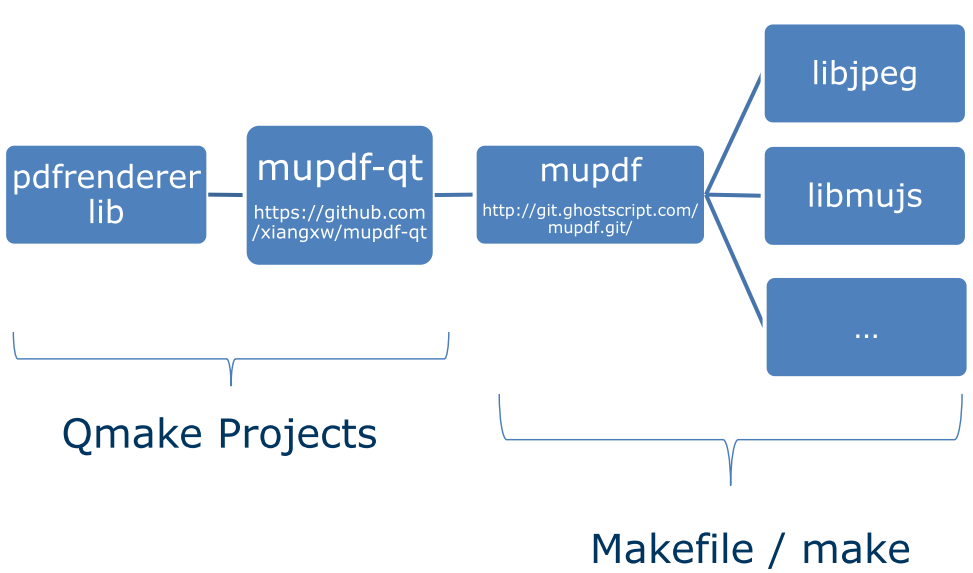
\includegraphics[angle=0,width=14cm]{PdfRenderer/pdfrenderer_aufbau.png}
\caption{Struktur und Aufbau des PDF-Renderer}
%\label{Ladeschluss}
\end{figure}


 

